\documentclass[border=10pt]{standalone}
\usepackage[T1]{fontenc}
\usepackage{tikz}
\usepackage[svgnames]{xcolor}
\usetikzlibrary{arrows.meta, positioning, calc, decorations.pathreplacing}

\colorlet{OrangeFill}{LightSalmon}
\colorlet{OrangeLine}{DarkSalmon!30!Chocolate}
\colorlet{GreenFill}{MediumAquamarine}
\colorlet{GreenLine}{MediumAquamarine!30!Teal}
\colorlet{PurpleFill}{MediumPurple}
\colorlet{PurpleLine}{MediumPurple!30!SlateBlue}
\colorlet{PinkFill}{Thistle}
\colorlet{PinkLine}{Thistle!30!Plum}
\colorlet{BlueFill}{LightSkyBlue}
\colorlet{BlueLine}{SteelBlue}
\colorlet{GrayFill}{LightGray!60!OldLace}
\colorlet{GrayLine}{RosyBrown!50!Silver}

\newcommand{\gridpt}[3]{% x, y, style
    \filldraw[#3] (#1,#2) circle (3pt);
}

\begin{document}
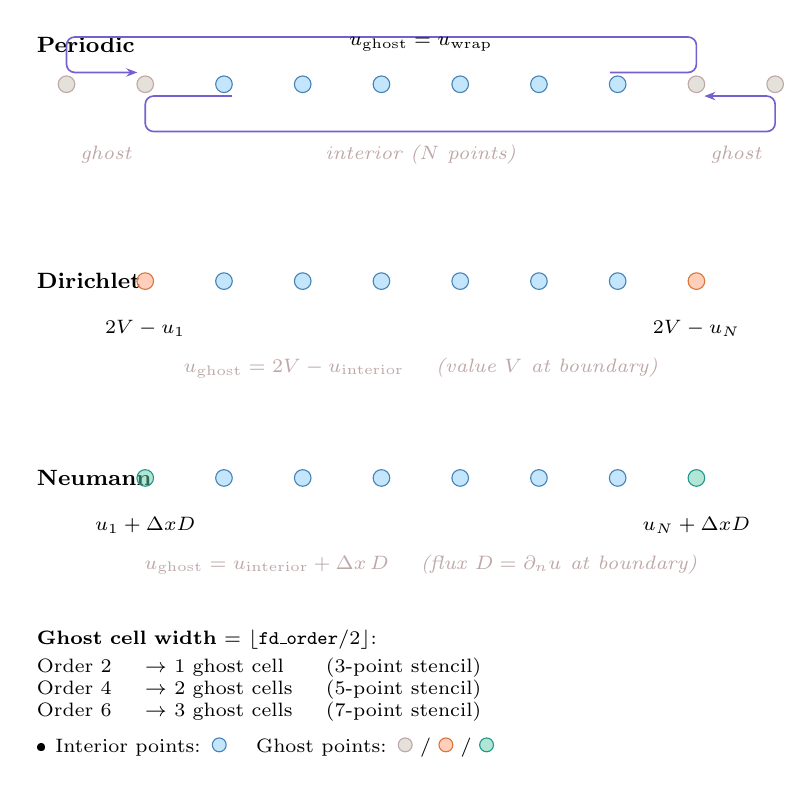
\begin{tikzpicture}[
    annot/.style={font=\scriptsize\itshape, text=GrayLine, align=center},
    lbl/.style={font=\scriptsize, text=black, align=center},
    arr/.style={-{Stealth[length=4pt, width=3pt]}, semithick},
    node distance=0.5cm
]

% ===================================================================
% PERIODIC BCs (top row)
% ===================================================================
\node[font=\footnotesize\bfseries, anchor=west] at (-1.5, 3.5) {Periodic};

% Ghost cells (left)
\gridpt{-1}{3}{GrayLine, fill=GrayFill}
\gridpt{0}{3}{GrayLine, fill=GrayFill}
% Interior
\foreach \x in {1,2,3,4,5,6} {
    \gridpt{\x}{3}{BlueLine, fill=BlueFill, fill opacity=0.5}
}
% Ghost cells (right)
\gridpt{7}{3}{GrayLine, fill=GrayFill}
\gridpt{8}{3}{GrayLine, fill=GrayFill}

% Wraparound arrows
\draw[arr, PurpleLine, rounded corners=3pt]
    (5.9,3.15) -- (7,3.15) -- (7,3.6) -- (-1,3.6) -- (-1,3.15) -- (-0.1,3.15);
\draw[arr, PurpleLine, rounded corners=3pt]
    (1.1,2.85) -- (0,2.85) -- (0,2.4) -- (8,2.4) -- (8,2.85) -- (7.1,2.85);

\node[lbl, above=0.3cm of {(3.5,3)}] {$u_{\mathrm{ghost}} = u_{\mathrm{wrap}}$};

% Labels
\node[annot] at (-0.5, 2.1) {ghost};
\node[annot] at (3.5, 2.1) {interior ($N$ points)};
\node[annot] at (7.5, 2.1) {ghost};

% ===================================================================
% DIRICHLET BCs (middle row)
% ===================================================================
\node[font=\footnotesize\bfseries, anchor=west] at (-1.5, 0.5) {Dirichlet};

% Ghost cells
\gridpt{0}{0.5}{OrangeLine, fill=OrangeFill, fill opacity=0.5}
% Interior
\foreach \x in {1,2,3,4,5,6} {
    \gridpt{\x}{0.5}{BlueLine, fill=BlueFill, fill opacity=0.5}
}
% Ghost cell
\gridpt{7}{0.5}{OrangeLine, fill=OrangeFill, fill opacity=0.5}

% Value annotations
\node[lbl] at (0, -0.1) {$2V - u_1$};
\node[lbl] at (7, -0.1) {$2V - u_N$};

\node[annot] at (3.5, -0.6) {$u_{\mathrm{ghost}} = 2V - u_{\mathrm{interior}}$
    \quad (value $V$ at boundary)};

% ===================================================================
% NEUMANN BCs (bottom row)
% ===================================================================
\node[font=\footnotesize\bfseries, anchor=west] at (-1.5, -2.0) {Neumann};

% Ghost cell
\gridpt{0}{-2.0}{GreenLine, fill=GreenFill, fill opacity=0.5}
% Interior
\foreach \x in {1,2,3,4,5,6} {
    \gridpt{\x}{-2.0}{BlueLine, fill=BlueFill, fill opacity=0.5}
}
% Ghost cell
\gridpt{7}{-2.0}{GreenLine, fill=GreenFill, fill opacity=0.5}

% Value annotations
\node[lbl] at (0, -2.6) {$u_1 + \Delta x D$};
\node[lbl] at (7, -2.6) {$u_N + \Delta x D$};

\node[annot] at (3.5, -3.1) {$u_{\mathrm{ghost}} = u_{\mathrm{interior}} + \Delta x\, D$
    \quad (flux $D = \partial_n u$ at boundary)};

% ===================================================================
% STENCIL ANNOTATION
% ===================================================================
\node[font=\scriptsize, align=left, text width=6.0cm,
      anchor=north west] at (-1.5, -3.8) {%
    \textbf{Ghost cell width} = $\lfloor\texttt{fd\_order}/2\rfloor$:\\[2pt]
    \begin{tabular}{@{}l l l@{}}
        Order 2 & $\to$ 1 ghost cell & (3-point stencil) \\
        Order 4 & $\to$ 2 ghost cells & (5-point stencil) \\
        Order 6 & $\to$ 3 ghost cells & (7-point stencil) \\
    \end{tabular}\\[4pt]
    \textbullet\ Interior points: \tikz\filldraw[BlueLine, fill=BlueFill,
        fill opacity=0.5] (0,0) circle (2.5pt); \quad
    Ghost points: \tikz\filldraw[GrayLine, fill=GrayFill] (0,0) circle (2.5pt);
    / \tikz\filldraw[OrangeLine, fill=OrangeFill, fill opacity=0.5]
        (0,0) circle (2.5pt);
    / \tikz\filldraw[GreenLine, fill=GreenFill, fill opacity=0.5]
        (0,0) circle (2.5pt);};

\end{tikzpicture}
\end{document}
